\documentclass[11pt, oneside]{article}   	% use "amsart" instead of "article" for AMSLaTeX format
\usepackage{geometry}                		% See geometry.pdf to learn the layout options. There are lots.
\geometry{letterpaper}                   		% ... or a4paper or a5paper or ...
%\geometry{landscape}                		% Activate for rotated page geometry
%\usepackage[parfill]{parskip}    		% Activate to begin paragraphs with an empty line rather than an indent
\usepackage{graphicx}				% Use pdf, png, jpg, or eps§ with pdflatex; use eps in DVI mode
								% TeX will automatically convert eps --> pdf in pdflatex
\usepackage{amssymb}
\usepackage{amsmath}
\usepackage{gensymb}

\usepackage{lmodern}
\usepackage[T1]{fontenc}
\usepackage[utf8]{inputenc}

%SetFonts

\title{Brief Article}
\author{The Author}
%\date{}							% Activate to display a given date or no date

\begin{document}

\section{Situation}

\subsection{Simulation}

La simulation se déroule sur un temps $T$ ($t \in [0, T[$).
La vitesse de rotation en longitude de la Terre est $v_{\mathit{Terre}}$.

\subsection{Des satellites}

On dispose de plusieurs satellites $S$ qui orbitent autour de la terre à
chaque intervalle de temps $t$. \\*

Chaque satellite $s \in S$ est défini par :

\begin{itemize}
\item sa position (latitude, longitude) au temps $t$ : $P_{s, t} = (\varphi_{s, t}, \lambda_{s, t})$
\item sa vitesse en latitude $v_{s, t}$ ($100 \leq |v_{s,t}| \leq 500$)
\item l'orientation de la caméra au temps $t$ : $(\Delta\varphi_{s, t}\, \Delta\lambda_{s, t})$
\item la vitesse maximale de rotation de la caméra sur les deux directions $w_s$
\item l'orientation maximale de la caméra dans les deux directions $d_s$
\end{itemize}

On peut mettre par écrit plusieurs équations qui définié
l'\'eaavolution de la caméra dans le temps, pour tout $t$ :

\begin{equation}
-d_s \leq \Delta\varphi_{s, t} \leq d_s
\label{max-phi}
\end{equation}

\begin{equation}
-d_s \leq \Delta\lambda{s, t} \leq d_s
\label{max-lambda}
\end{equation}

\begin{equation}
\Delta\varphi_{s, t+1} \in [-w_s\Delta\varphi_{s, t}, w_s\Delta\varphi_{s, t}]
\label{max-speed-phi}
\end{equation}

\begin{equation}
\Delta\lambda_{s, t+1} \in [-w_s\Delta\lambda_{s, t}, w_s\Delta\lambda_{s, t}]
\label{max-speed-lambda}
\end{equation}

L'évolution de la position du satellite $s$ dans le temps, pour tout $t$ :

\begin{equation}
\begin{displaystyle}
\text{La latitude } \varphi_{s, t+1} =
	\begin{cases}
		\varphi_{s, t} + v_s & \mathit{si} -90\degree \leq \varphi_{s, t} + v_s \leq 90\degree \\
		180\degree - (\varphi_{s, t} + v_s) & \mathit{si} \ \varphi_{s, t} + v_s > 90\degree \footnotemark \\
		-180\degree - (\varphi_{s, t} + v_s) & \mathit{si} \ \varphi_{s, t} + v_s < -90\degree \footnotemark \\
	\end{cases}
\end{displaystyle}
\end{equation}

\addtocounter{footnote}{-1}
\footnotetext{On passe par dessus le pôle Nord}
\stepcounter{footnote}
\footnotetext{On passe par dessus le pôle Sud}

\begin{equation}
\begin{displaystyle}
\text{La longitude }\lambda_{s, t+1} =
	\begin{cases}
		\lambda_{s, t} + v_{Terre} & \mathit{si} -90\degree \leq \varphi_{s, t} + v_s \leq 90\degree \\
		-180\degree - (\lambda_{s, t} + v_{Terre}) & \mathit{si} \ \varphi_{s, t} + v_s > 90\degree \\
		-180\degree - (\lambda_{s, t} + v_{Terre}) & \mathit{si} \ \varphi_{s, t} + v_s < -90\degree
	\end{cases}
\end{displaystyle}
\end{equation}

\begin{equation}
\begin{displaystyle}
\text{La vitesse } v_s =
	\begin{cases}
		v_s & \mathit{si} -90\degree \leq \varphi_{s, t} + v_s \leq 90\degree \\
		-v_s & \mathit{si} \ \varphi_{s, t} + v_s > 90\degree \\
		-v_s & \mathit{si} \ \varphi_{s, t} + v_s < -90\degree
	\end{cases}
\end{displaystyle}
\end{equation}

\subsection{Des collections}

On dispose d'une liste de collections $C$. \\

Chaque collection $c \in C$ est définie par :

\begin{itemize}
\item une valeur de score $score_c$
\item une liste de points à capturer  $P_c = [(\varphi_1, \lambda_1), (\varphi_2, \lambda_2), ...]$
\item une liste d'intervalles de temps dans lesquels il est possible de capturer les points
$R_c = [[t_1, t_2], [t_3, t_4], ...]$
\end{itemize}

%-----------------

\section{Le problème}

Posons $X$ la listes des points capturés : $X = [(x, s, t),
...]$\footnote{Ici un point $x = (\varphi, \lambda)$ capturé par le satellite $s$ au temps $t$}

On cherche à maximiser le score avec

\begin{equation}
	\mathit{score} = \sum_{c \; \in \; C_{\mathit{prises}}} \mathit{score}_c
\end{equation}

$C_{\mathit{prises}}$ représente les collections ``prises'', c'est à dire
les collections dont on a photographié tous les points.

\begin{equation}
	C_{\mathit{prises}} = \{ c \ | \ c  \in  C \; \mathit{et} \ \forall p \in P_{c} \ \exists (x, s, t) \in X \ \mathit{tq} \ x = p \}
\end{equation}

o\`u

$C$ : l'ensemble des collections

$P_{c}$ : les points de la collection $c$

$X$ : les points capturés \\

Définissons $X$, l'ensemble des points capturés :

\begin{equation}
	X = \{ p \ | \ p \ \in \ \underset{c \ \in \ C}\cup P_{c} \ \mathit{et} \ p
    \;  \text{``a été capturé''} \}
\end{equation}

On dit que $p$ ``a été capturé'' si :

\begin{equation}
	\exists s \in S, \ \exists t \in [0, \, t_{max}[ \ \mathit{tel \, que} \ p = (\varphi_{s, t} + \Delta\varphi_{s, t}, \, \lambda_{s, t} + \Delta\lambda_{s, t})
\end{equation}

\emph{ie.} il existe un satellite $s$ qui a prit $p$ en photo au temps $t$.


\textbf{Les seules variables du problème sont donc les orientations des
caméras à chaque tour $t$.}

\subsection{Taille du problème}

Pour $N$ satellites pendant $T$ tours il y a donc $N \times T \times
2$ variables\footnote{2 pour les positions $\Delta\varphi$ et $\Delta\lambda$}.
Calculons le nombre de positions différentes de caméra.

\begin{table}[htb]
\begin{center}
\begin{tabular}{ l | r r r r }
    Jeu & \emph{constellation} & \emph{forever alone} & \emph{overlap} &
    \emph{weekend} \\
	\hline
    N     & 25         & 1         & 32         & 40         \\
    T     & 259 200    & 604 800   & 604 800    & 172 800    \\
    total & 12 960 000 & 1 209 600 & 38 707 200 & 13 824 000 \\
\end{tabular}
\end{center}
\caption{\label{tab:taille}Tailles du problème.}
\end{table}


% --------

\section{Idées}

\subsection{Algorithme génétique}

Puisque que les seules valeurs que nous pouvons influencer concernent
l'orientation de la caméra de chaque satellite, les solutions au problème
ressemblent à la liste des mouvements des caméras permettant d'effectuer le
meilleur score. \\

Pour chaque caméra, on peut donc créer une table comme montré à la figure
\ref{tab:mouvements}. \footnote{Vu la taille du problème - plusieurs millions
de lignes - l'implématation matérielle gagnera a être différente et ne pas
stocker les lignes qui ne font rien.}

\begin{table}[htb]
\begin{center}
\begin{tabular}{ l | r r}
	temps & Décalage $\Delta\varphi$ & Décalage $\Delta\lambda$ \\
	\hline
 	0 & 0 & 0 \\
	1 & +2 & -1 \\
	2 & +10 & -1 \\
	 \multicolumn{3}{l}{...} \\
	T-1 & -2 & +3 \\
\end{tabular}
\end{center}
\caption{\label{tab:mouvements}Mouvements de la caméra du satellite 1.}
\end{table}

On créerait donc des individus possédant autant de tables qu'il y a de
satellites et on les ferait évoluer à la recherche d'une solution optimale.

Les décalages $\Delta\varphi$ et $\Delta\lambda$ ne prennent pas n'importe
quelle valeur. On doit respecter les contraintes exprimées dans les
équations \eqref{max-phi} \eqref{max-lambda} \eqref{max-speed-phi}
\eqref{max-speed-lambda}. \\

\subsubsection{Fonction d'évalutation}

La fonction d'évaluation n'est pas complexe. Elle consiste à faire tourner
la simulation en appliquant les mouvements de caméra, observer les points
capturés et calculer les scores.

\subsubsection{Mutations et croisements}

Problème ici.

Une mutation peut consister en l'addition ou la soustraction de $1$ sur une case
d'une des tables d'un individu, tant que la nouvelle position n'entraine pas de
situation interdite.

Le croisement pose problème car on va certainement créer une solution
interdite.
L'idée la plus simple pour croiser deux individus $x_1$ et $x_2$ est
de sélectionner un m\^eme satellite $s$ dans chaque et de croiser les table
de mouvements liées (\emph{ie} les découper au temps $t_k$ et échanger deux
morceaux afin de créer $x_1'$ et $x_2'$). La ligne $t_{k+1}$ dans les tables
est probablement incompatible avec la ligne $t_k$ (vitesse trop grande,
dépassement de la borne $d_s$).

\subsubsection{Modéliser les mouvements par un graphe}

Figure \ref{fig:graph} à garder en t\^ete.

\begin{figure}[htb]
    \begin{center}
        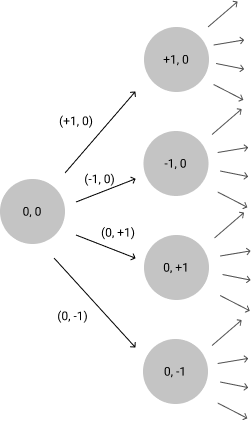
\includegraphics[scale=0.5]{graph.png}
        \caption{\label{fig:graph}Modélisation des valeurs que peut prendre une
        ligne de la table \ref{tab:mouvements}}
    \end{center}
\end{figure}

En fonction du mouvement précédent, certains mouvement deviennent interdits car
ils vont mettre en défaut les équations \eqref{max-phi} \eqref{max-lambda}
\eqref{max-speed-phi} \eqref{max-speed-lambda}.

\subsection{Recuit simulé}

Cette fois-ci, on cherche à faire évoluer qu'un seul individu $x_i$.

Comme pour l'idée de l'algorithme génétique, on crée des tables de
mouvements pour chaque caméra de chaque satellite.
On utilise la même fonction d'évaluation que pour l'algorithme génétique

\subsubsection{Transformation}

$x_0$ a donc toutes ses tables à 0. Il faut décider de la transformation à
appliquer. Comme pour l'algorithme génétique, on peut appliquer un décalage sur
$\Delta\varphi$ ou $\Delta\lambda$ à un instant $t$ aléatoire.

\end{document}
